\chapter{Environment Influence } 
Not just the sample rate and error is determining factors when designing a \ab{NILM} application. The environment which the application is deployed and trained in is critical for the performance of the system. 

The environment is the parameters describing the static conditions of the household which the algorithms is deployed in. An example of an environment parameter can be number of known devices, number of unknown devices, number of simultaneously active devices or number of training days. In order to investigate some of the environment parameters effect the SmartHG dataset is used. 

\section{Challenges In The SmartHG Dataset} 
The \ab{ECO} dataset, consists of 6 households and the data is sampled at a rate of 1 Hz over a period of 8 months. The SmartHG dataset is different in many aspects. The data is sampled at a slower rate of $\frac{1}{30}$ Hz, but on 25 households over a period of 6 month. Each house have only a small number of sub-meters. The sub-meters is mainly placed on little consumers such as televisions and stereos, which presents an interesting challenge for load disaggregation. The SmartHG dataset contains both the aggregated data, and the instantaneous power usages of the different households.

\begin{figure}[H]
\centering
\includegraphics[width=1\textwidth]{billeder/TotalPie.png}
\caption{Frequency comparison of the reconstruction methods}
\label{fig:SLC}
\end{figure}

In figure \ref{fig:SLC} is the power distribution of three households shown. This illustrates how much energy each appliance uses, in relation to the households total energy consumption. The Other category shows the energy consumption not accounted for by the sub-meters.  

Household 3,10 and 18 is some of the houses that have the smallest "other" category. They are therefore selected for further study, since they provide the most information about the house. 

\section{Appliance Noise Influence On Detection }
The households in the SmartHG dataset have a relative big consumption created by other appliances than the ones with a sub-meter. The consumption can be thought of as "appliance noise", since it is a signal that is not included in the disaggregation model. 

\subsection{Detection In A Noisy Environment }
To investigate the influence appliance noise have on a \ab{NILM} application, disaggregation of the known appliances of house 3, 10 and 18 is done using the Parson and \ab{FHMM} algorithm. 

\begin{table}[H]                             
\centering                                   
\begin{tabular}{c|c|c|c|c|}  
\cline{2-5}                                      
 & \multicolumn{2}{|c|}{FHMM} & \multicolumn{2}{c|}{Parson} \\                      
\cline{2-5}                                        
 & F1 & Accuracy & F1 & Accuracy \\          
\hline                                       
\multicolumn{1}{|c|}{TV 1 }& 0.19 & 0.74 & 0.10 & 0.40 \\          
\hline                                       
\multicolumn{1}{|c|}{PC }& 0.19 & 0.84 & 0.13 & 0.45 \\            
\hline                                       
\multicolumn{1}{|c|}{TV 2 }& 0.03 & 0.84 & 0.20 & 0.11 \\          
\hline                                       
\multicolumn{1}{|c|}{\textbf{Average House 3 }}& \textbf{0.14} & \textbf{0.81} & \textbf{0.14} & \textbf{0.32} \\ 
\hline                                       
\multicolumn{1}{|c|}{TV 1} & 0.60 & 0.76 & 0.40 & 0.25 \\          
\hline                                       
\multicolumn{1}{|c|}{Stereo }& - & 1.00 & - & 1.00 \\              
\hline                                       
\multicolumn{1}{|c|}{PC }& - & 0.99 & - & 0.99 \\                  
\hline                                       
\multicolumn{1}{|c|}{TV 2 }& - & 0.99 & - & 0.99 \\                
\hline                                       
\multicolumn{1}{|c|}{\textbf{Average House 10}} & \textbf{0.15} & \textbf{0.94} & \textbf{0.10} & \textbf{0.81} \\
\hline                                       
\multicolumn{1}{|c|}{TV 1} & 0.36 & 0.65 & 0.24 & 0.14 \\          
\hline                                       
\multicolumn{1}{|c|}{Lamp} & - & 0.99 & - & - \\                   
\hline                                       
\multicolumn{1}{|c|}{TV 2} & 0.73 & 0.58 & - & 0.00 \\             
\hline                                       
\multicolumn{1}{|c|}{\textbf{Average House 18} }& \textbf{0.36} & \textbf{0.74} & \textbf{0.08} & \textbf{0.04} \\
\hline                                       
\end{tabular}                                
\caption{Appliance disaggregation results of house 3,10 and 18 for the smartHG dataset}                     
\label{table:Tab:SHGREAL}                    
\end{table}  

On table \ref{table:Tab:SHGREAL} is the results from the disaggregation shown. The low F1 scores indicates that it is hard for the algorithms to correctly disaggregate the meters. This is due to the many spikes there are in the data that can indicate a \lipsum[1]

\begin{figure}[H]
\centering
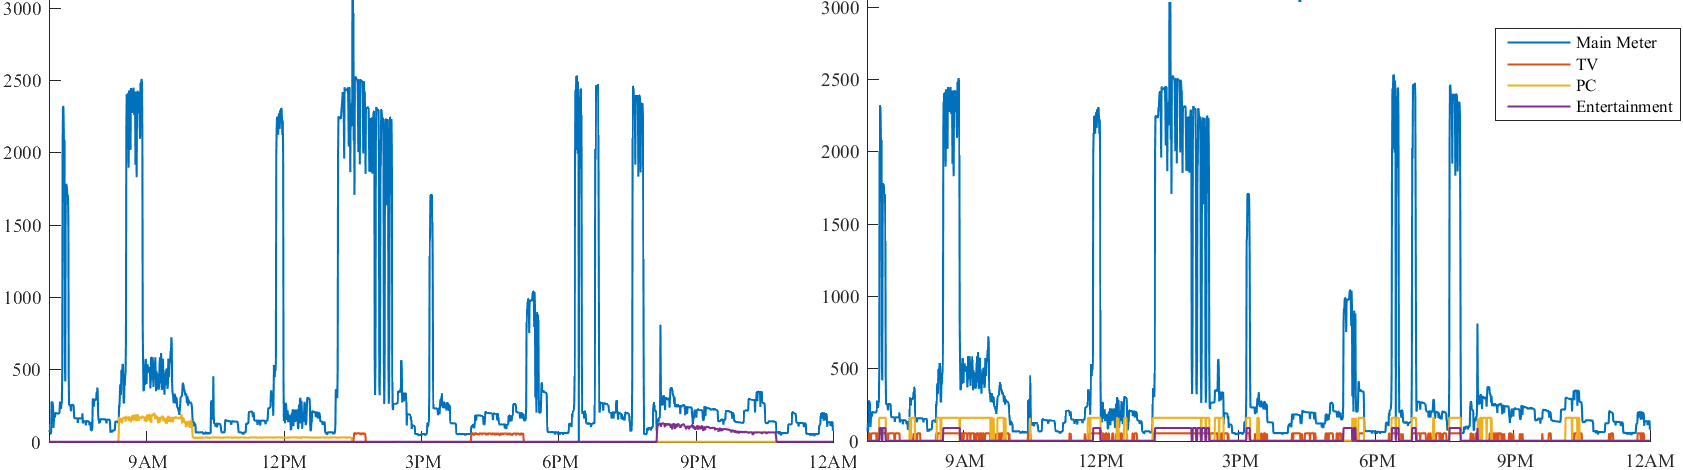
\includegraphics[width=1\textwidth]{billeder/RecognitionEx1.png}
\caption{}
\end{figure}


\subsection{Detection In Noise Free Environment }

\begin{table}[H]                             
\centering                                   
\begin{tabular}{|c|c|c|c|c|}                 
\hline                                       
 & F1 & Accuracy & F1 & Accuracy \\          
\hline                                       
TV 1 & 0.73 & 0.96 & 0.26 & 0.86 \\          
\hline                                       
PC & 0.74 & 0.96 & 0.30 & 0.91 \\            
\hline                                       
TV 2 & 0.83 & 0.96 & 0.20 & 0.11 \\          
\hline                                       
Total House 3 & 0.77 & 0.96 & 0.26 & 0.62 \\ 
\hline                                       
TV 1 & 0.97 & 0.98 & 0.40 & 0.25 \\          
\hline                                       
Stereo & - & 1.00 & - & 1.00 \\              
\hline                                       
PC & - & 0.99 & - & 0.99 \\                  
\hline                                       
TV 2 & - & 0.99 & - & 0.99 \\                
\hline                                       
Total House 10 & 0.24 & 0.99 & 0.10 & 0.81 \\
\hline                                       
TV 1 & 0.95 & 0.98 & 0.24 & 0.14 \\          
\hline                                       
Lamp & - & 0.99 & - & - \\                   
\hline                                       
TV 2 & 0.73 & 0.58 & 0.73 & 0.58 \\          
\hline                                       
Total House 18 & 0.56 & 0.85 & 0.32 & 0.24 \\
\hline                                       
\end{tabular}                                
\caption{MyTableCaption}                     
\label{table:Tab:SHGSIM}                     
\end{table} 

\subsection{Noise Effect On Training And Validation }

\begin{table}[H]                             
\centering                                   
\begin{tabular}{c|c|c|c|c|}                 
\hline                                       
 & F1 & Accuracy & F1 & Accuracy \\          
\hline                                       
TV 1 & 0.02 & 0.94 & 0.23 & 0.86 \\          
\hline                                       
PC & 0.29 & 0.94 & 0.32 & 0.92 \\            
\hline                                       
TV 2 & 0.00 & 0.88 & 0.20 & 0.11 \\          
\hline                                       
Total House 3 & 0.11 & 0.92 & 0.25 & 0.63 \\ 
\hline                                       
TV 1 & 0.00 & 0.74 & 0.40 & 0.25 \\          
\hline                                       
Stereo & - & 1.00 & - & 1.00 \\              
\hline                                       
PC & - & 0.99 & - & 0.99 \\                  
\hline                                       
TV 2 & - & 0.99 & - & 0.99 \\                
\hline                                       
Total House 10 & 0.00 & 0.93 & 0.10 & 0.81 \\
\hline                                       
TV 1 & 0.00 & 0.86 & 0.24 & 0.14 \\          
\hline                                       
Lamp & - & 0.99 & - & - \\                   
\hline                                       
TV 2 & 0.73 & 0.58 & 0.73 & 0.58 \\          
\hline                                       
Total House 18 & 0.24 & 0.81 & 0.32 & 0.24 \\
\hline                                       
\end{tabular}                                
\caption{MyTableCaption}                     
\label{table:Tab:SHGREALSIM}                 
\end{table}    


\begin{table}[H]                             
\centering                                   
\begin{tabular}{|c|c|c|c|c|}                 
\hline                                       
 & F1 & Accuracy & F1 & Accuracy \\          
\hline                                       
TV 1 & 0.10 & 0.42 & 0.10 & 0.45 \\          
\hline                                       
PC & 0.13 & 0.39 & 0.12 & 0.44 \\            
\hline                                       
TV 2 & 0.21 & 0.35 & 0.20 & 0.11 \\          
\hline                                       
Total House 3 & 0.15 & 0.39 & 0.14 & 0.33 \\ 
\hline                                       
TV 1 & 0.40 & 0.25 & 0.40 & 0.25 \\          
\hline                                       
Stereo & - & 1.00 & - & 1.00 \\              
\hline                                       
PC & - & 0.99 & - & 0.99 \\                  
\hline                                       
TV 2 & - & 0.99 & - & 0.99 \\                
\hline                                       
Total House 10 & 0.10 & 0.81 & 0.10 & 0.81 \\
\hline                                       
TV 1 & 0.27 & 0.26 & 0.24 & 0.14 \\          
\hline                                       
Lamp & - & 0.99 & - & - \\                   
\hline                                       
TV 2 & 0.73 & 0.58 & 0.73 & 0.58 \\          
\hline                                       
Total House 18 & 0.33 & 0.61 & 0.32 & 0.24 \\
\hline                                       
\end{tabular}                                
\caption{MyTableCaption}                     
\label{table:Tab:SHGSIMREAL}                 
\end{table}     

\subsection{ Model Size Influence }

\begin{figure}[H]
\centering
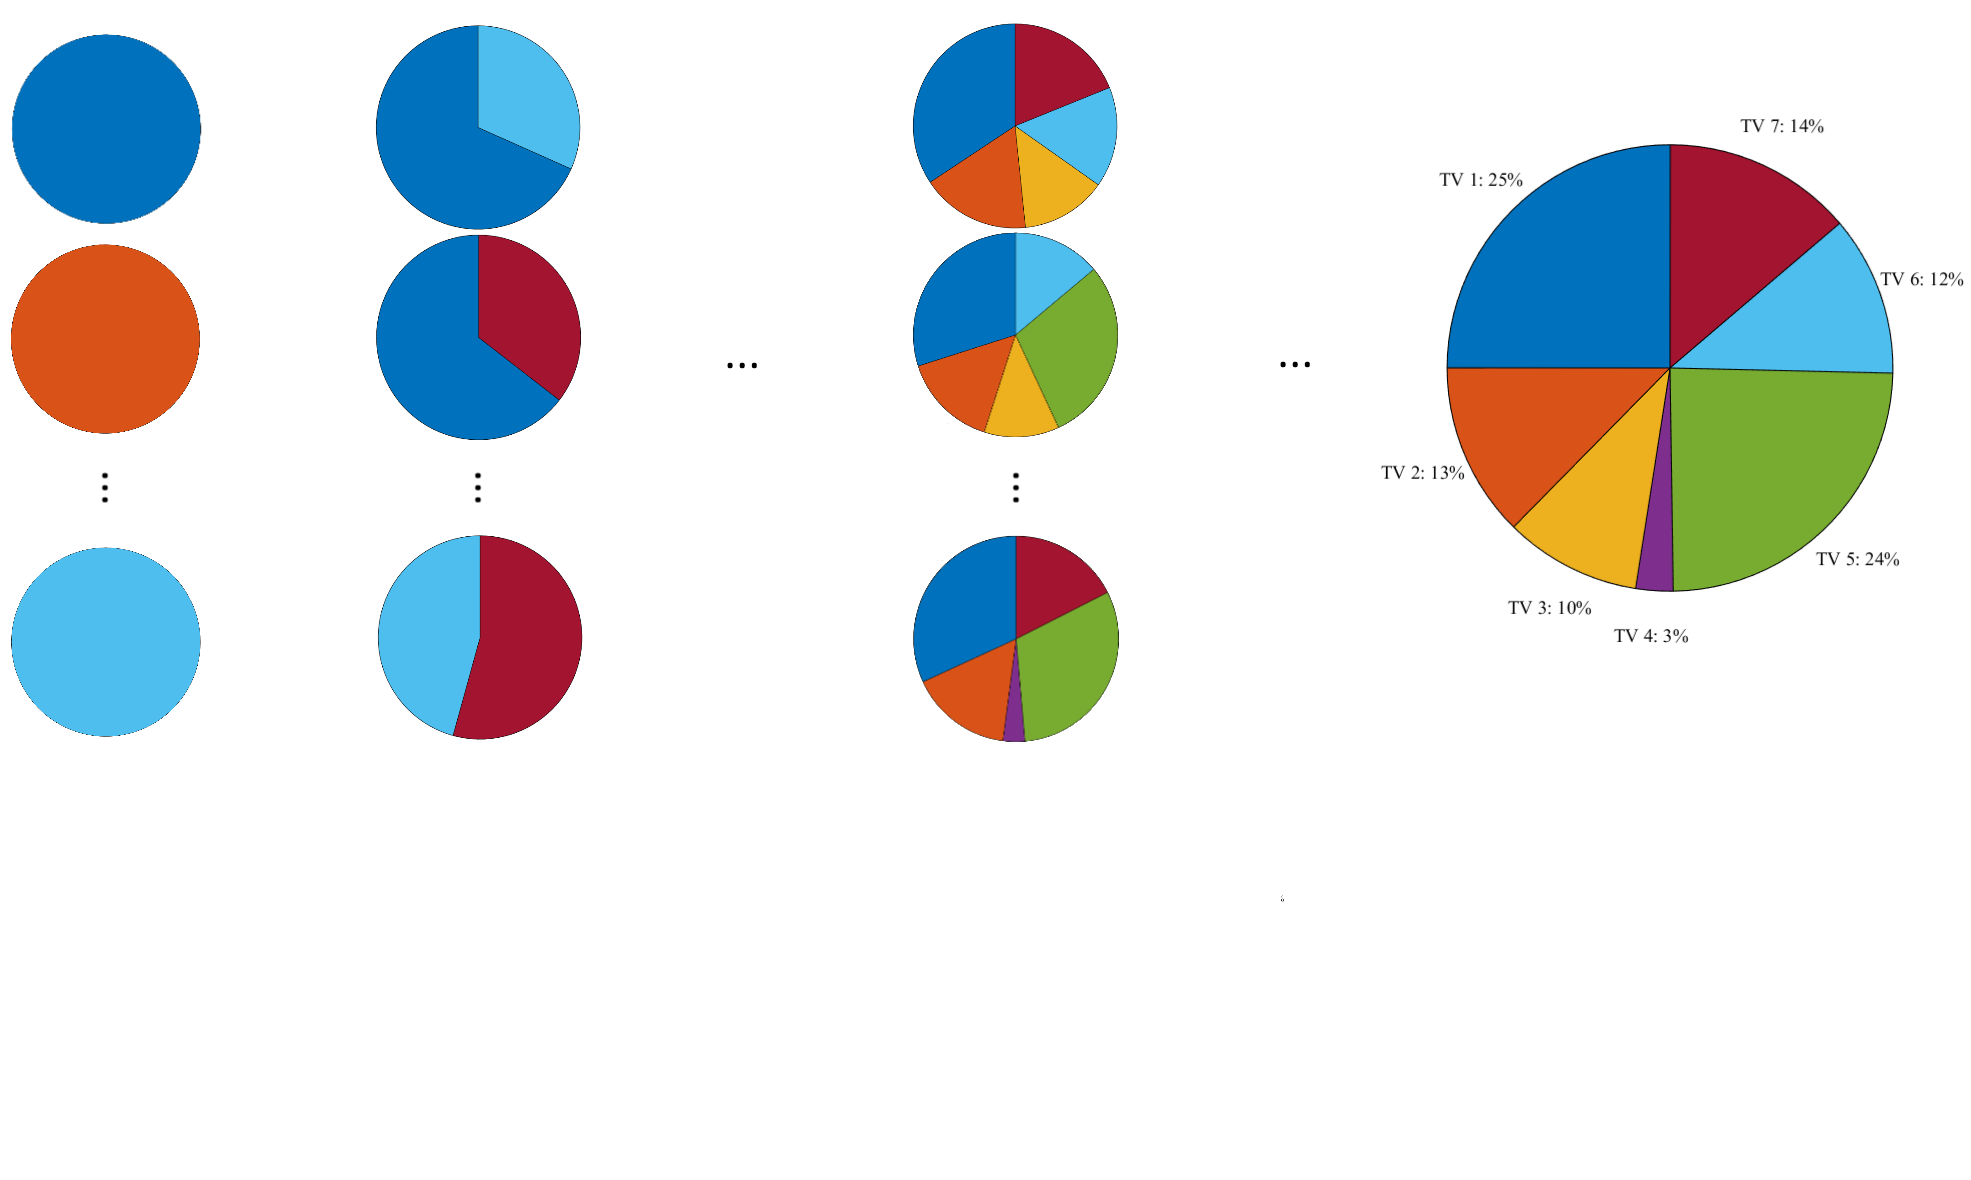
\includegraphics[width=1\textwidth]{billeder/CombiShow.png}
\caption{}
\end{figure}


\begin{figure}[H]
\centering
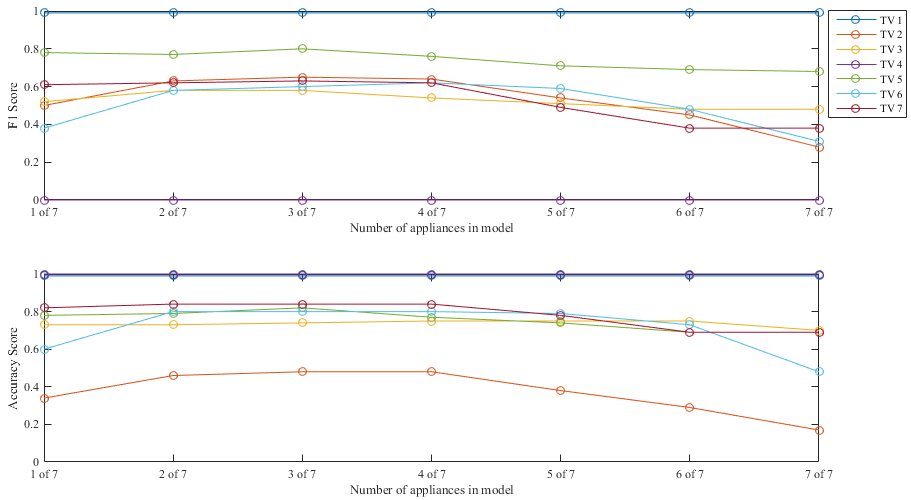
\includegraphics[width=1\textwidth]{billeder/ModelCompletness.png}
\caption{}
\end{figure}

\subsection{ Model Completeness Influence }

\begin{figure}[H]
\centering
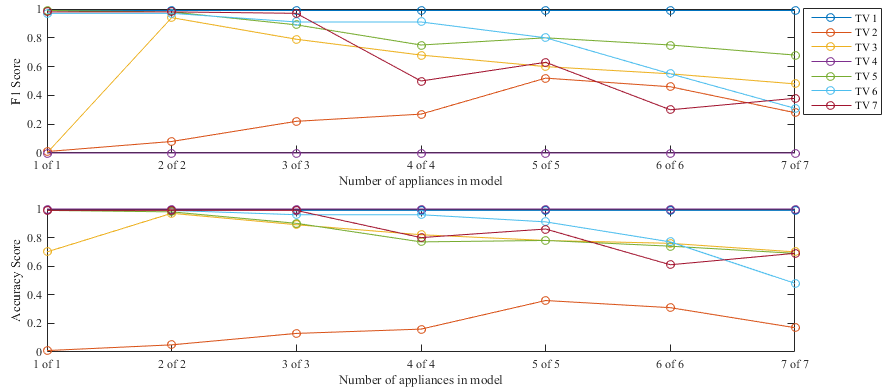
\includegraphics[width=1\textwidth]{billeder/ModelSize.png}
\caption{}
\end{figure}